\newcommand*{\mtol}{This is some more text than fit at ony line but only some   and not a lot}
\newenvironment{mldescription}{%   
\begin{addmargin}[2.5em]{0em}     
\setlength{\parindent}{-2.5em}%     
\newcommand*{\mlitem}[1]{\par\textbf{##1}\quad}\indent 
}{%   
\end{addmargin}   
\medskip }


\chapter{Enfoque y Herramientas\label{chap:Enfoque-y-Herramientas}}

En este capítulo se describe el enfoque propuesto para predecir atributos
dinámicos de componentes de software, en base a propiedades medidas
durante su ejecución. El enfoque plantea llevar a cabo la predicción
mediante un proceso de aprendizaje de máquina que involucra dos pasos:
medición y aprendizaje. El primero implica la recolección de indicadores
o mediciones durante la ejecución del componente, lo que puede significar
la ejecución de una pieza de código, la llamada a una función, o la
invocación de un servicio. Lo segundo implica la construcción de
modelos de predicción con técnicas de regresión. La construcción o
entrenamiento de estos modelos se hace en un proceso interactivo con
el usuario, que involucra una configuración inicial de los datos y
la optimización automática de los parámetros de acuerdo a las tasas
de error arrojadas por métricas de evaluación . Por último, los modelos
generados pueden utilizarse en distintos casos prácticos, como por
ejemplo, la selección automática de servicios y algoritmos, o soportar
decisiones de diseño o implementación. 

Como soporte para el enfoque, se desarrollaron dos herramientas independientes
diseñadas para efectuar cada uno de los pasos mencionados. Por un
lado, el framework\emph{ Android Meter} es una biblioteca Java para
realizar pruebas de desempeños de código en Android y capturar mediciones
durante la ejecución. Su diseño es genérico para usar sobre cualquier
dominio del que se quieran obtener mediciones de desempeño. Por otro
lado, se desarrolló una herramienta standalone denominada \emph{Nekonata}
diseñada para integrar fácilmente técnicas de aprendizaje automático
incluidas en librerías Java de terceros. La herramienta se usa para
la construcción del modelo a partir del conjunto de datos capturados
con el uso del framework Android Meter, mediante un proceso de automatización
de los algoritmos en complemento de información gráfica para la colaboración
interactiva del usuario. 

Estas cuestiones se describen en detalle de la siguiente manera. En
la sección \ref{sec:Etapas-del-m=0000E9todo} se profundiza sobre
las distintas etapas del enfoque, incluyendo algunos usos prácticos
de la propuesta. En las siguientes secciones se describen cada uno
de las herramientas desarrolladas, presentando el framework para la
medición y recolección de datos en la sección \ref{subsec:Framework-de-medici=0000F3n}
y finalmente, en la sección \ref{subsec:Herramienta-de-entrenamiento}
se presenta la herramienta para la construcción de modelos de predicción. 


\section{Etapas del método\label{sec:Etapas-del-m=0000E9todo}}

El enfoque propuesto se conceptualiza como un proceso de dos fases
complementarias, con las que se obtienen modelos de predicción de
propiedades de componentes que pueden usarse en distintas aplicaciones
o casos prácticos. La figura \ref{fig:method-stages} muestra un esquema
conceptual del enfoque, cuyas etapas se describen a continuación:

\begin{figure}
\begin{centering}
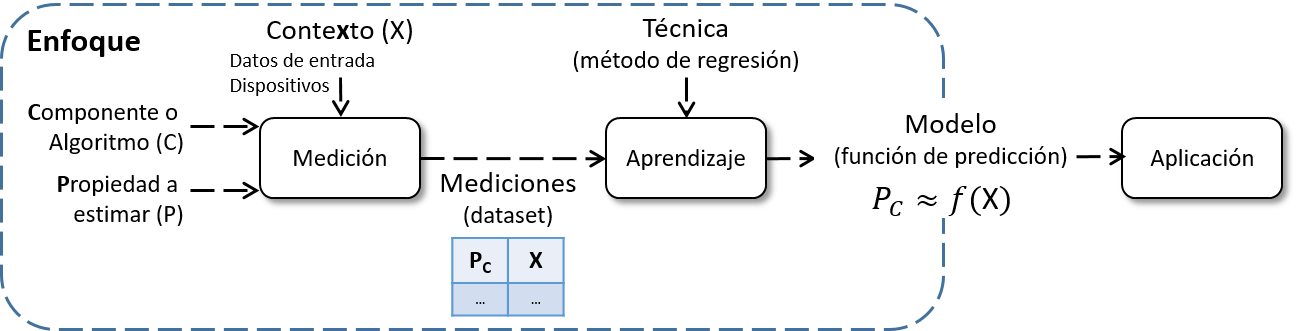
\includegraphics[scale=0.55]{images/enfoque-overview}
\par\end{centering}

\caption{Esquema conceptual del enfoque en fases. \label{fig:method-stages}}
\end{figure}



\subsection*{Medición y recolección de datos }

\noindent El proceso comienza con la medición de un componente en
ejecución y la recolección de estas mediciones en un dataset. Cada
dataset pertenece a la ejecución de un componente diferente, del cual
se extraen todas sus mediciones de desempeño (tiempo de respuesta,
etc) mas las propiedades que podrían influir sobre este desempeño.
Durante la ejecución de cada componente se van realizando las mediciones
sobre distintos aspectos de la operación y registrando cada uno de
estos resultados en un archivo para su posterior análisis. A su vez,
el proceso de recolección de datos involucra la ejecución de sub etapas,
pudiendo requerir el proceso algunas o todas las tareas que se detallan
a continuación:
\begin{itemize}
\item Integración de componentes: A menudo se requiere la evaluación de
componentes de terceros, tanto de servicios Web como algoritmos de
bibliotecas instaladas, de manera que deben ser integrados correctamente
a la herramienta para ser tratados como componentes. 
\item Selección de características del contexto: mientras se realiza la
ejecución de los componentes, las características del dispositivo
móvil donde se llevan a cabo las operaciones pueden ser capturadas
como mediciones. Realizar las mediciones sobre distintos dispositivos
móviles persigue la idea de que las capacidades de cada dispositivo
(cantidad de memoria, CPU, etc) influye en el desempeño de los componentes,
como por ejemplo, su tiempo de ejecución.
\item Generación de datos de entrada: los componentes requieren un conjunto
de parámetros o datos de entrada para su ejecución, por eso se debe
proveer una manera para generar arbitrariamente instancias de datos
de entrada del componente a medir, o la capacidad para obtener instancias
externamente a través de enlaces o archivos. 
\item Selección de propiedades de la entrada: Es posible obtener propiedades
de los datos de entrada, generalmente atributos que configuran o sirven
para generar una instancia como su tamaño. 
\item Ejecución de componentes y obtención de mediciones: los componentes
son ejecutados con las entradas generadas, mientras se toman y registran
mediciones sobre las propiedades del contexto de ejecución (datos
de entrada y dispositivo), que son los atributos independientes o
predictores, además de las propiedades de interés a predecir. De esta
forma, el dataset que se obtiene puede ser formado por una cantidad
variable de propiedades en base a las características que hayan sido
elegidas para ser medidas. 
\end{itemize}

\subsection*{Aprendizaje}

A partir del conjunto de datos obtenidos en la etapa anterior, se
aplican técnicas de aprendizaje de máquina para la extracción de conocimiento.
Tal conocimiento se refleja mediante la construcción de modelos predictivos
que mejor se ajustan a la generalización de la información mediante
un proceso de entrenamiento, optimización y evaluación de los mismos.
El proceso de aprendizaje requiere indefectiblemente de un conjunto
de datos de entrenamiento volcado en un archivo, una propiedad de
ese conjunto a predecir y un conjunto de algoritmos que aplican técnicas
de regresión sobre los datos. El aprendizaje está conformado por varias
sub etapas o sub procesos.
\begin{itemize}
\item Configuración de las técnicas: las técnicas de regresión representan
algoritmos que pueden involucrar diferentes parámetros de configuración.
La variabilidad en estos valores permite ajustar las preferencias
del algoritmo y consecuentemente, la obtención de modelos de calidad
diferente. Por lo tanto, el desafío principal de esta parte de la
etapa es encontrar los valores apropiados para cada uno de los parámetros,
teniendo como base, el conocimiento sobre el efecto que el parámetro
causa en el algoritmo. Al obtener la mejor configuración de una técnica,
para un dataset y una propiedad particular, se facilita la comparación
simultánea de todas las técnicas disponibles a través de las métricas
de evaluación y en consecuencia seleccionar la más óptima. 
\item Construcción de modelos: la construcción o entrenamiento de modelos
predictivos es un proceso que implica la ejecucion de una o mas técnicas
de regresión sobre el conjunto de los datos y continúa opcionalmente
con un proceso de evaluación.El entrenamiento utiliza las mediciones
ya obtenidas en la etapa anterior y a partir de la propiedad que se
desea predecir, el algoritmo va definiendo la función o modelo de
regresión que mejor ajusta las relaciones entre los atributos independientes
(o predictores) del dataset y el atributo a predecir. Esta etapa concentra
el mayor porcentaje del tiempo computacional y uso de memoria, y varía
de acuerdo a la complejidad o simplicidad de cada técnica en particular. 
\item Evaluación de modelos: una vez concluida la etapa de entrenamiento,
el modelo obtenido puede ser analizado para determinar la medida en
que este es capaz de generalizar cualquier entrada de dataset futura
y estimar la propiedad de interés. La noción sobre el desempeño del
modelo tiene lugar a partir de métricas existentes para modelos de
regresión, que capturan el error de predicción o el coeficiente de
correlación para conocer el grado de interdependencia de las propiedades. 
\end{itemize}

\subsection*{Aplicaciones de los modelos\label{sec:Aplicaciones-de-la-1}}

Finalmente, se pretende utilizar estos modelos de predicción en entornos
de aplicación que permitan la selección del componente más adecuado
en base a propiedades de los parámetros de entrada u otras propiedades
del contexto de ejecución, a través de un proceso automatizado que
determine al usuario la opción más favorable evitando la ejecución
individual de cada componente.  La construcción de modelos de predicción
de performance ha ido creciendo debido a la utilidad que presentan
en una gran variedad de contextos prácticos. A continuación, se detallan
algunos:
\begin{description}
\item [{Selección~de~algoritmos}] Como se ha tratado en algunos trabajos
\citet{Hutter2014}, los modelos de predicción son útiles para la
selección automática de algoritmos . A través de estos modelos se
puede predecir con cierto error el rendimiento de cada uno de estos
algoritmos candidatos y mediante una simple comparación seleccionar
el más apropiado considerando la instancia del problema y las características
del hardware. 
\item [{Ajustes~de~parámetros~y~configuración~automática~del~algoritmo}] Los
modelos predictivos sirve a dos propósitos fundamentales. Por un lado,
modelar el comportamiento o funcionalidad de un algoritmo parametrizado
en base a la configuración de tales parámetros, en cuyo caso se puede
alternar entre el aprendizaje del modelo y su uso para identificar
configuraciones interesantes para evaluar posteriormente. Por otro
lado, se puede modelar el rendimiento del algoritmo basado conjuntamente
en las características de las instancias del problema y la configuración
de sus parámetros. Tales modelos pueden utilizarse para ajustar los
valores de tales parámetros y obtener una mejor predicción basada
en la instancia particular. 
\end{description}
\begin{mldescription} 
\mlitem{Obtener una visión general de las instancias y el rendimiento de los algoritmos} Los modelos se pueden utilizar para evaluar las características de la instancia y los valores de los parámetros del algoritmo que más impactan en el rendimiento. Algunos modelos son compatibles con este tipo de evaluaciones directamente. Para otros modelos, existen métodos de selección de atributos (características genéricas) para identificar un grupo más reducido de entradas del modelo que son claves, y describen el rendimiento del algoritmo casi tan bien como todo el conjunto de entradas.
\end{mldescription} 
\begin{description}
\item [{Selección~de~servicio~para~composición~de~servicios}] Cuando
varios servicios Web implementan la misma funcionalidad, los modelos
de rendimiento resultan ser un buen criterio para escoger el mejor
candidato entre ellos. Incluso en tiempo de ejecución, los proveedores
de servicio pueden cambiarse si las condiciones del contexto y los
parámetros de entrada se modifican. 
\item [{Planificación~de~tareas~en~redes~móviles}] Suponiendo un conjunto
de tareas que deben asignarse entre un conjunto de dispositivos, los
modelos de rendimiento podrían obtener una medida aproximada del tiempo
de respuesta que cada tarea requerirá sobre cada dispositivo con el
fin de minimizar el tiempo total de secuenciación de las tareas.
\end{description}

\section{Framework de medición para Android\label{subsec:Framework-de-medici=0000F3n}}

\emph{Android Meter} es un framework diseñado para simplificar la
medición de propiedades de performance de componentes ejecutados bajo
el sistema Android. El framework esta implementado como una biblioteca
Java que permite ejecutar diferentes piezas de software y capturar
propiedades y mediciones durante su ejecución. La biblioteca ofrece
el soporte necesario para adaptarla a distintos dominios de componentes
y algoritmos, y recolectar las mediciones que sirven de fuente para
construir modelos de predicción a través de técnicas de aprendizaje
de máquina. 

El framework se basa en el concepto central de \emph{Componente},
que representa cualquier entidad de ejecución, como una funcion, algoritmo
o servicio, que provee una funcionalidad a través de una interfaz
específica. 

\begin{figure}
\begin{centering}
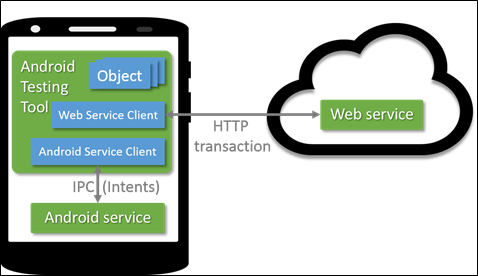
\includegraphics[scale=0.7]{images/android-component}
\par\end{centering}

\caption{Esquema conceptual de componentes Android considerados. \label{fig:android-component}}
\end{figure}


En la figura \ref{fig:android-component} se ilustran distintos tipos
de componentes que se pueden ejecutar y medir desde el framework,
incluyendo servicios Web, servicios específicos de la plataforma Android,
y cualquier algoritmo o pieza de código que se implemente como metodos
de objetos Java. Las instancias de objetos hacen referencia a cualquier
componente residente en el espacio de memoria de una aplicación, el
componente específico para servicios web incluye cualquier componente
remoto fuera del dispositivo y accedidos a través de protocolos de
comunicación Web, como \ac{HTTP}. Por último el componente específico
para servicios Android incluye cualquier proceso ejecutado en segundo
plano residente en el mismo dispositivo y accedidos a través de objetos
Intent (mecanismo de comunicación entre procesos del sistema Android). 

A continuación se expone en la figura \ref{fig:TestingTool-Diagram}
los principales conceptos que forman parte al framework \emph{Android
Meter}. 

\begin{figure}
\begin{centering}
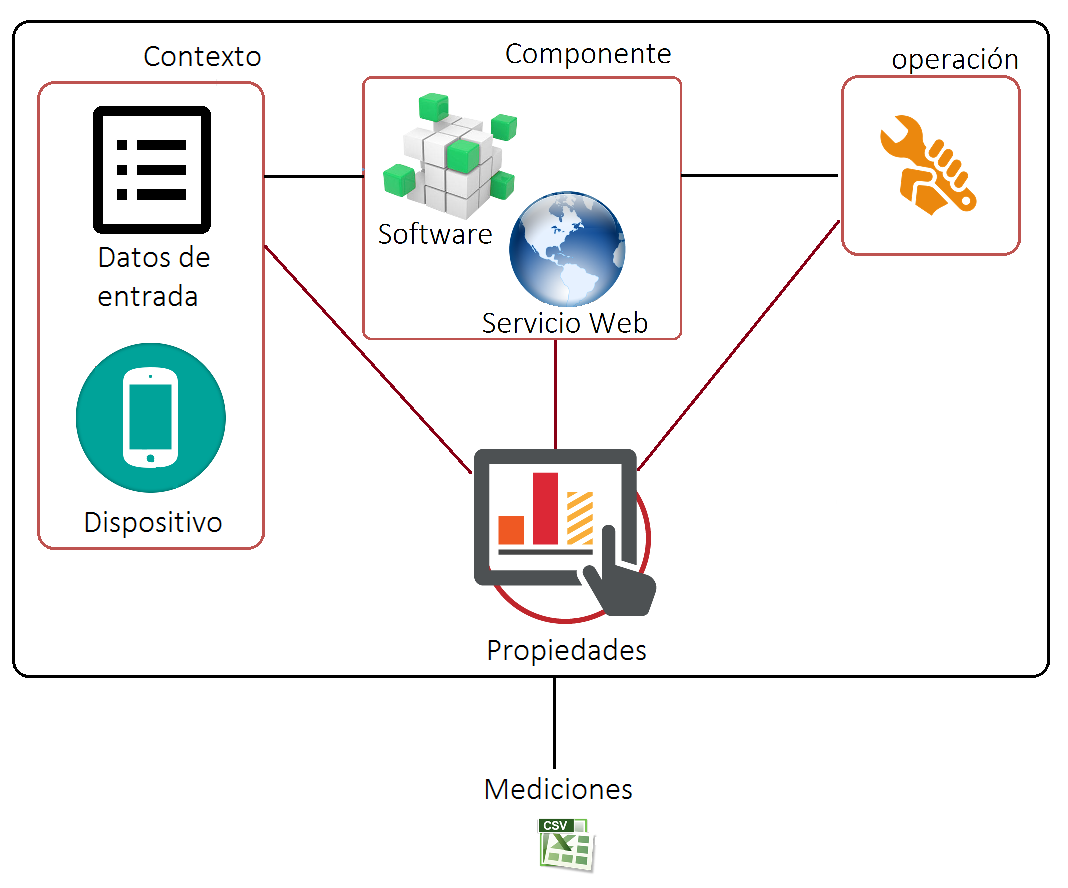
\includegraphics[scale=0.33]{images/TestingTool-Diagram}
\par\end{centering}

\caption{Conceptos principales del framework Android Meter.\label{fig:TestingTool-Diagram}}
\end{figure}


La obtención de diferentes conjuntos de mediciones se realiza a través
de la creación de planes de pruebas, que se configuran y posteriormente
se ejecutan para obtener los datasets. Al momento de configurar los
planes de pruebas se tiene la posibilidad de especificar qué componentes
se ejecutarán, con qué datos de entrada, y qué propiedades o métricas
se desean capturar, ya sean propiedades del contexto, de los datos,
o propiedades no funcionales de la ejecución de los componentes. Las
propiedades a obtener pueden ser:
\begin{enumerate}
\item Propiedades del contexto: son las cualidades del entorno de ejecución,
es decir, el dispositivo sobre el que se ejecuta la prueba de performance.
Estas propiedades pueden ser estáticas, es decir, que se mantienen
sin cambio durante la ejecución del plan de pruebas, como por ejemplo,
el modelo del dispositivo, la arquitectura y cantidad de núcleos del
CPU, tamaño de memoria, etc; y dinámicas, que son las propiedades
del entorno que pueden variar durante la ejecución de los componentes,
como el uso de CPU, el número de procesos en ejecución, tipo de conexión,
etc. 
\item Propiedades de los datos de entrada: son atributos que se pueden extraer
de los parámetros con los que se invocan los componentes. Por ejemplo,
dado un algoritmo de ordenamiento de vectores, el tamaño del vector
de entrada seria una de estos atributos.
\item Propiedades del componente: atributos del componente como el nombre,
ubicación, etc.
\item Propiedades no funcionales: son las propiedades de interés que se
desean inferir a partir de las propiedades anteriores. Estas propiedades
se capturan en cada operacion de componentes, es decir, la ejecucion
de un componente con determinados datos de entrada. Por ejemplo, el
tiempo de respuesta, el consumo de batería, si la operación fue ejecutada
con éxito o con error, etc.
\end{enumerate}

\section{Herramienta de aprendizaje de modelos\label{subsec:Herramienta-de-entrenamiento}}

Nekonata es una herramienta para la construcción de modelos predictivos
a través de técnicas de aprendizaje de máquina. El eje que ha guiado
el diseño de la herramienta ha sido el brindar soporte para el uso
de cualquier librería que ofrezca aprendizaje de máquina a través
de la implementación de todos los conceptos involucrados como objetos
independientes a los cuales adaptar las funcionalidades de las librerías.
La herramienta \emph{Nekonata} lleva a cabo dos tipos de procesos
en el desarrollo de sus funciones: procesos automáticos y procesos
semi-automáticos que requieren la colaboración del usuario con el
fin de mejorar los resultados a partir de vistas gráficas que visualizan
el comportamiento y características de los modelos y además, para
incluir en el proceso el interés y criterio del usuario. 

El flujo de trabajo de la herramienta consta de dos etapas, una de
configuración y entrenamiento de modelos y otra de evaluación de los
mismos. 

\begin{figure}
\begin{centering}
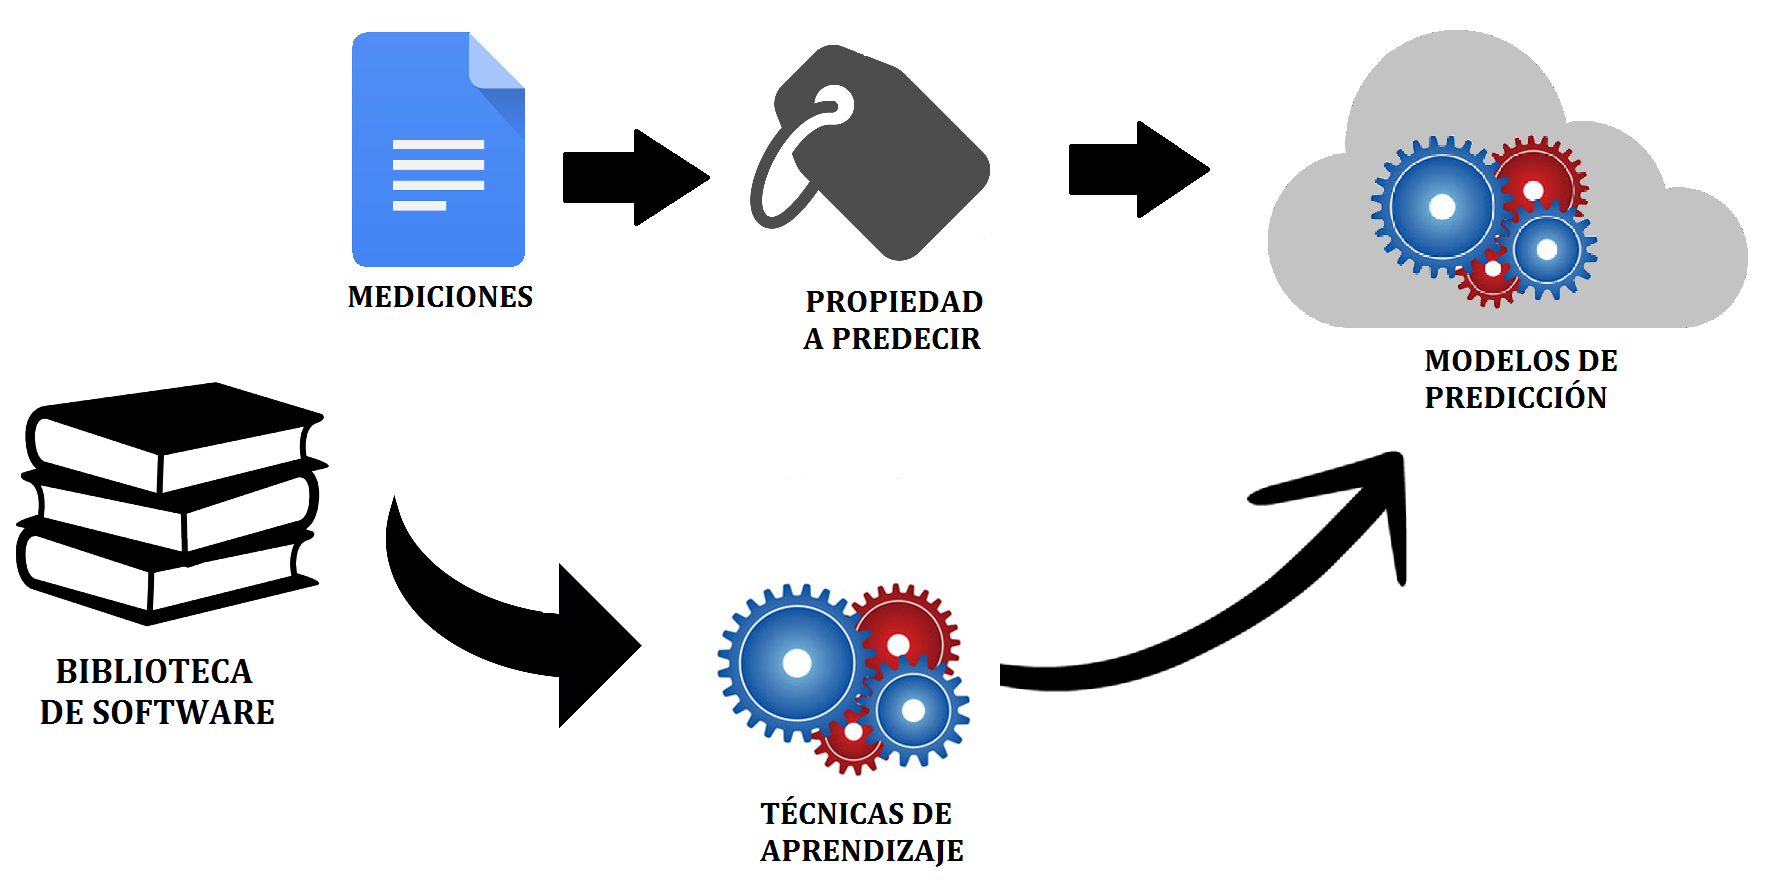
\includegraphics[scale=0.2]{images/prediction-workflow}
\par\end{centering}

\caption{Diagrama de flujo del proceso de configuración y entrenamiento de
modelos.\label{fig:prediction-workflow-1}}
\end{figure}


En la etapa de configuración, se indican la biblioteca y el dataset
que se desea considerar, habilitando la elección de las técnicas de
aprendizaje y de la propiedad dinámica a predecir. Una vez seleccionados
todos los valores requeridos, se procede a ejecutar las técnicas de
aprendizaje para generar los modelos de predicción. Un detalle importante
a considerar es que la herramienta no sólo genera los modelos a partir
de parámetros fijos, sino que realiza una comparación interna entre
modelos parciales para la obtención de una función de predicción más
precisa y acertada.

Luego de la etapa de entrenamiento, los modelos generados por cada
técnica son expuestos a una serie de métricas dispuestas de manera
tal que permita visualizar las diferencias de desempeño entre técnicas
con la misma métrica de evaluación considerada. Esta vista es un recurso
ofrecido al usuario para decidir aquel modelo que a su criterio tenga
mejor calidad a través de la comparación simultánea. Estas métricas
de evaluación incluyen: el coeficiente de correlación de Pearson (CC)
y la raíz del error cuadrático medio (RMSE).

\begin{figure}
\begin{centering}
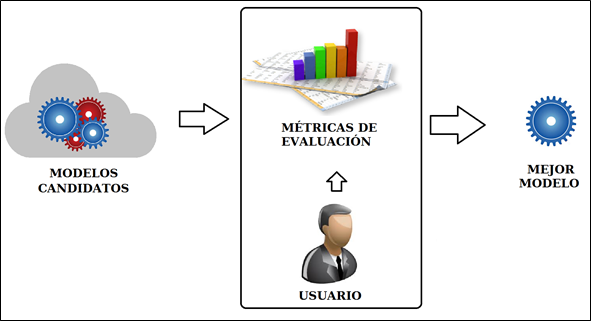
\includegraphics[scale=0.55]{C:/Users/usuario/Tesisworkspace/Tesis_Standalone/tesis/images/models-comparison-workflow}
\par\end{centering}

\caption{Diagrama de flujo de la fase de comparación de modelos. \label{fig:models-comparison-workflow}}
\end{figure}


Es conveniente trasladar el análisis a la mayor cantidad de métricas
posibles, ya que un mismo indicador podría arrojar valores cercanos
entre un algoritmo y otro favoreciendo equivocadamente a uno de ellos,
error que podría notarse al compararlos simultáneamente con otras
métricas. La metodología de operación de esta fase se muestra en la
figura \ref{fig:models-comparison-workflow}. 

\begin{figure}
\begin{centering}
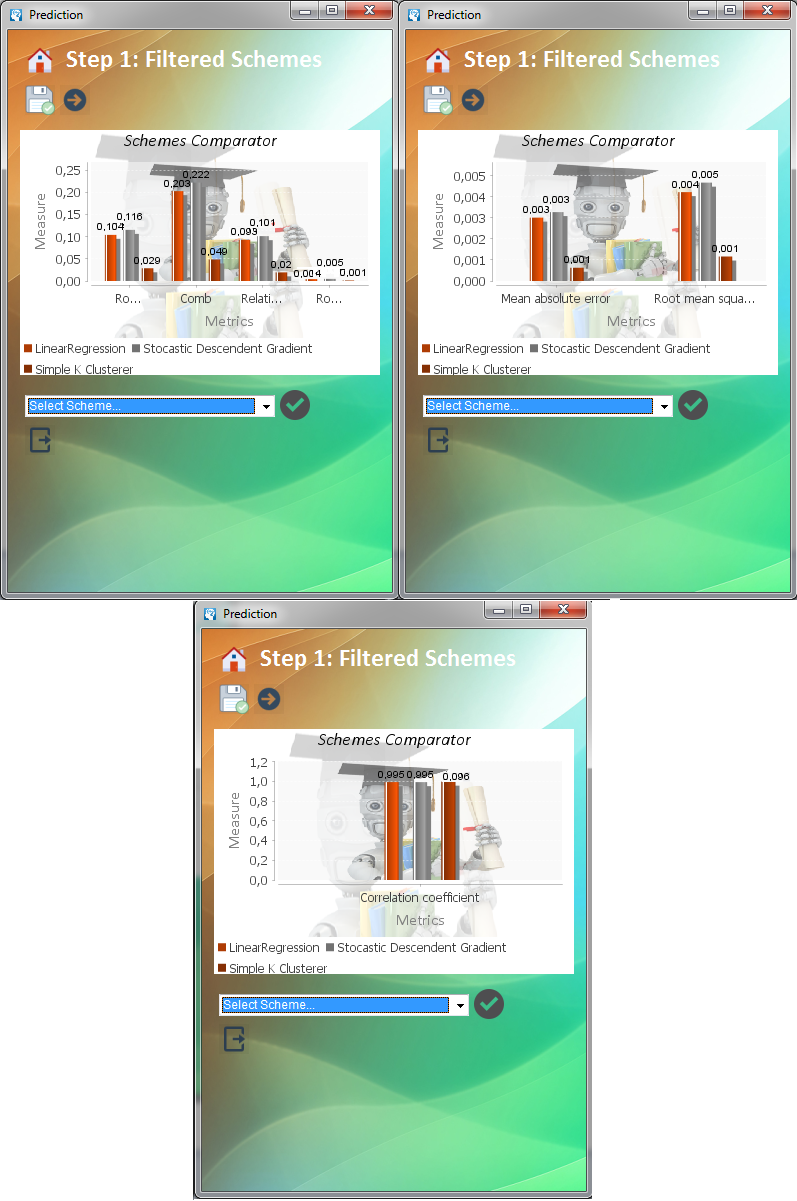
\includegraphics[scale=0.45]{images/errors_screenshot}
\par\end{centering}

\caption{Captura de pantalla de la herramienta \label{fig:models-comparison-workflow-1}}
\end{figure}


Nekonata hace foco en este detalle y ofrece al usuario una vista de
imágenes (\ref{fig:models-comparison-workflow-1})con los indicadores
medidos de cada algoritmo seleccionado por el usuario para aplicar
el proceso de optimización y elegir, posteriormente, el que resulte
más adecuado. La información gráfica complementaria que se brinda,
detalla los algoritmos representados por medio de barras y agrupados
en categorías separadas de acuerdo a cada métrica a modo de facilitar
la comparación. Adicionalmente las barras se colorean en dos tonos
diferentes para acentuar, por cada métrica, los clasificadores que
significarían las mejores opciones para ese indicador. 

La herramienta se desarrolló como una aplicación de escritorio pensada
para desarrolladores e ingenieros de datos que necesitan un entorno
usable y eficiente para construir modelos de predicción y analizar
los datos . Esta implementación desvincula el framework de medición
con la herramienta de aprendizaje, permitiendo la ejecución independiente
entre ambas, y el puente de comunicación entre ellas es la correspondencia
entre la salida de la primer herramienta con la entrada de la segunda.

El atributo principal que dirigió el diseño de la herramienta fue
la extensibilidad de la misma. Esto significa que la herramienta puede
aceptar diferentes tipos de bibliotecas de aprendizaje de máquina,
datasets, modelos de regresión, parámetros y métricas. Esto se logró
con una implementación orientado a objetos y basada en patrones de
diseño.

Actualmente, la aplicación ofrece una implementación de las siguientes
técnicas de regresión considerando la biblioteca de software Weka:
\begin{itemize}
\item Linear Regression: Es la implementación de la técnica Lineal Regression,
considerando la variante de Ridge Regression.
\item Neural Network Regression: Es la implementación de la técnica de Neural
Network, considerando la variante de Multilayer Perceptron.
\item Stochastic Gradient Descendent: Es la implementación de la técnica
de Lineal Regression, considerando la variante de gradiente descendiente
o SGD.
\item Support Vector Machine Regression: Es la implementación de la técnica
Vector Machine, considerando la variante de Sequential Minimal Optimization.
\item Simple K Clusterer: Es una adaptación de la técnica de clustering
K-Means Clusterer para regresión.
\end{itemize}
A través del uso de métricas se adquiere una idea estimativa del desempeño
del clasificador frente al conjunto de datos de entrenamiento, sin
embargo, podría resultar útil conocer el comportamiento general del
algoritmo, contrastando cada uno de los valores reales del atributo
clase con los valores predichos por el clasificador, y obtener así
una vista exacta de la manera en que el clasificador se ajusta a los
datos (Figura \ref{fig:screenshot-error-curve}). 

Este recurso es usado en la herramienta como un gráfico de dos líneas
continuas de distinto color para representar el conjunto de datos
de entrenamiento y el conjunto de datos predichos. Cada punto del
dominio corresponde a cada instancia y la unión entre puntos sólo
se realiza con fines ilustrativos. 

\begin{figure}
\begin{centering}
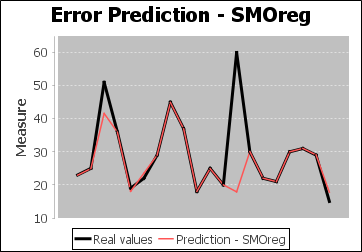
\includegraphics[scale=0.8]{images/screenshot-error-curve}
\par\end{centering}

\caption{Captura de pantalla de la vista del error de predicción. \label{fig:screenshot-error-curve}}
\end{figure}

